In order to assess how the identified models generalize into a situation with wind, predictions have been conducted for an idealization of a wind state. The idealized wind state is a very simplified hydrodynamic condition where the models have a drift angle, but no yaw rate or rudder angle. This is meant to represent a state where the ship is experiencing a static drift angle for a long time -- induced by a side wind force.
The prediction results for the idealized wind condition are shown in \autoref{fig:result_wind_state}. The yawing moment $N_D$ is highly under predicted by the Abkowitz ID compared to the Reference model. This is because most of the yawing moment is denoted to the yaw rate coefficients $N_r,N_{rrr}$ (as previously stated in \autoref{sec:result_ID_regression}) -- which are not activated in the wind state. The Physics informed ID identified by inverse dynamics regression does not seem to have the same problem, where $N_D$ is much closer to the Reference model. Both of the ID models seem to under predict the sway force $Y_D$ a bit.
\label{sec:wind_state}
\begin{figure}[h!]
    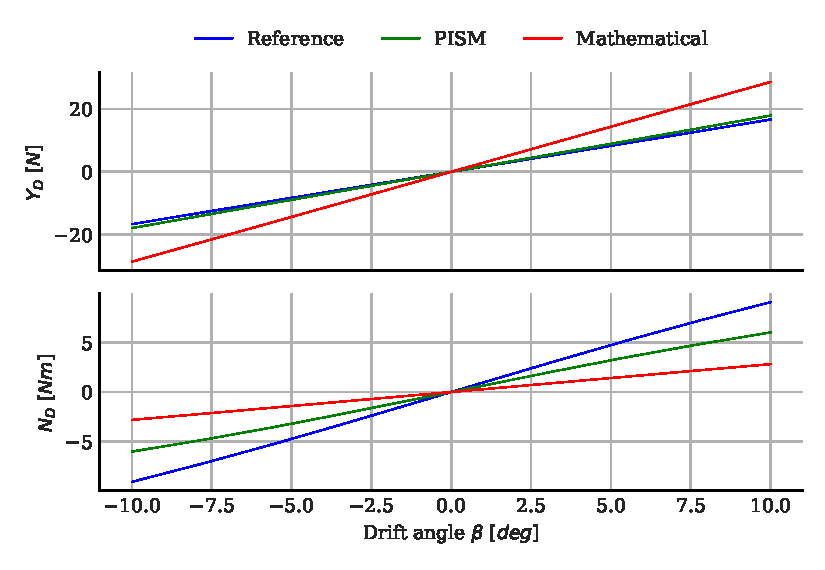
\includegraphics[width=\columnwidth]{figures/result_wind_state.forces.pdf}
    \caption{Total sway force and yawing moment from the models at various drift angles.}
    \label{fig:result_wind_state}
\end{figure}